\documentclass[11pt]{article}
\usepackage[margin=1in]{geometry}
\usepackage{amsfonts, amsmath, amssymb}
\usepackage[none]{hyphenat}
\usepackage{fancyhdr}
\usepackage{graphicx}
\usepackage{float}
\usepackage[nottoc, notlot, notlof]{tocbibind}
\usepackage{apacite}
\usepackage[bottom]{footmisc}
\usepackage[italian]{babel}

\pagestyle{fancy}
\fancyhead{}
\fancyfoot{}
\fancyhead[L]{\slshape \MakeUppercase{Network Alignment}}
\fancyhead[R]{\slshape Luca Masiero, Stefano Ivancich}
\fancyfoot[C]{\thepage}
%\renewcommand{\headrulewidth}{0pt}
\renewcommand{\footrulewidth}{0pt}

%\parindent 0ex per l'indendazione
%\setlength{\parindent}{4em}
%\setlength{\parskip}{1em}
%\renewcommand{\baselinestretch}{1.5}
\begin{document}

\begin{titlepage}
\begin{center}
\vspace*{1cm}
\Large{\textbf{Università degli Studi di Padova}}\\
\Large{\textbf{Corso di Laurea Magistrale in Ingegneria Informatica}}\\
\begin{center}

\includegraphics[scale=0.2]{uni}
\end{center}
%\vfill
\line(1,0){470}\\[1mm]
\Huge{\textbf{\begin{huge}Progetto di \textit{Algoritmi per la Bioinformatica}\end{huge}}}\\[3mm]
\Huge{\textbf{Network Alignment}}\\[1mm]
\Large{\textbf{- PPI: Protein-Protein Interaction -}}\\[1mm]
\line(1,0){270}\\
\begin{flushright}
\textbf{Studenti}: \textit{Luca Masiero}\\\textit{Stefano Ivancich}
\end{flushright}

\begin{flushleft}
\textbf{Supervisor}: \textit{Prof. Matteo Comin}\\
\end{flushleft}
\vfill
\textbf{Anno Accademico 2019-2020}
 \\
18 Giugno 2020
\end{center}
\end{titlepage}
\setcounter{page}{1}
\newpage
\begin{titlepage}
\begin{center}
\vspace*{1cm}
\vfill
\begin{flushright}
\small{\textit{L'unica maniera per scoprire i limiti del possibile è avventurarsi poco al di là di essi nell'impossibile.}}\\
\small{Arthur C. Clarke}\\
\end{flushright}
\vfill
\end{center}
\end{titlepage}
\tableofcontents %compila due volte per l'indice corretto!
\thispagestyle{empty}
\clearpage

\newpage
\section{Introduzione: \textit{Network Alignment} e \textit{PPIN}}
L'obiettivo del \textit{\textbf{Network Alignment}} (traducibile con \textit{allineamento delle reti}) consiste nel trovare somiglianze tra la struttura e/o la topologia di due o più reti. 

Nel contesto biologico, confrontare le reti di diversi organismi (rappresentate tramite \textit{grafi}) è, attualmente, uno dei problemi più importanti ed interessanti della Biologia. Gli allineamenti di reti biologiche possono infatti risultare molto utili perché, avendo molte informazioni su alcuni nodi di una determinata rete $G_1$ e quasi nulla su nodi topologicamente simili in un'altra $G_2$, la conoscenza specialistica di uno di quei nodi può dirci qualcosa di nuovo sul corrispettivo. Gli allineamenti delle reti possono anche essere utilizzati per misurare la somiglianza globale tra reti complete di specie diverse. 

Le \textit{\textbf{Protein-Protein Interaction Networks}} (\textbf{PPIN}, \textit{reti di interazione proteina-proteina}) sono strumenti validi per comprendere le funzioni delle cellule, le malattie umane e il design e riposizionamento dei farmaci\footnote{Il \textit{drug-repositioning} è l’insieme delle analisi volte a stabilire se un farmaco già noto possa essere utilizzato per il trattamento di sintomatologie diverse da quelle descritte in etichetta.}; nonché per ottenere una descrizione completa degli \textit{interattomi}\footnote{Si veda la \textit{\textbf{Sottosezione 2.1.}}} affinché sia possibile capire, tramite la loro analisi comparativa, più profondamente i processi biologici.

\begin{center}
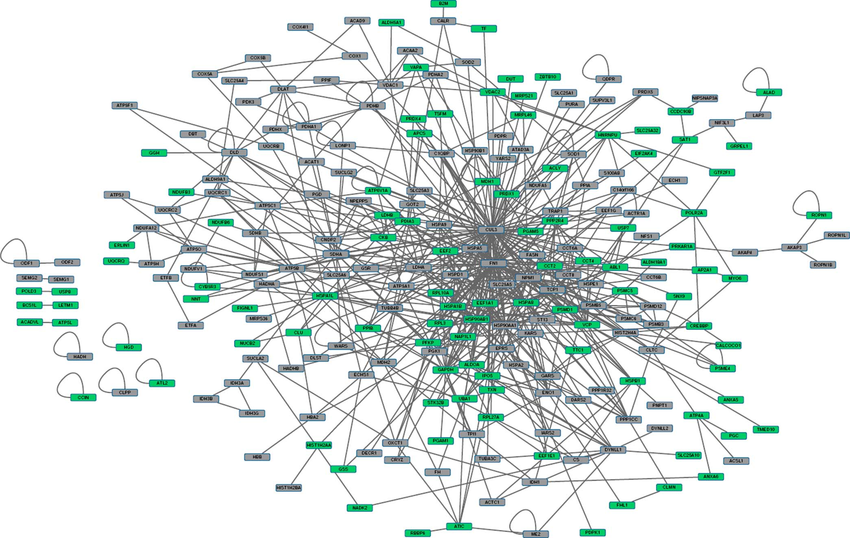
\includegraphics[scale=0.46]{woo}

\begin{small}\textit{\textbf{Figura 1.1}: Un esempio di PPIN.}\end{small}
\end{center}

Interpretare una PPI è un compito particolarmente impegnativo a causa della complessità della rete. Negli anni, sono stati proposti diversi algoritmi per l'interpretazione automatica delle PPI, in un primo momento considerando esclusivamente la \textit{topologia della rete}\footnote{La topologia di rete è il modello (grafo) finalizzato a rappresentare le relazioni di connettività, fisica o logica, tra gli elementi costituenti la rete stessa (i \textit{nodi}).}, e successivamente integrando i termini dell'\textit{Ontologia Genica}\footnote{Nato nel 1988, \textit{Gene Ontology} è un progetto bioinformatico atto a unificare la descrizione delle caratteristiche dei prodotti dei geni in tutte le specie. In particolare, il progetto si propone di: 
\begin{enumerate}
\setlength{\itemsep}{1pt}
  \setlength{\parskip}{0pt}
  \setlength{\parsep}{0pt}
\item Mantenere e sviluppare un vocabolario controllato atto a descrivere i geni e i prodotti genici per ogni organismo vivente;
\item Annotare i geni e i prodotti genici, e diffondere tali dati;
\item Fornire strumenti per un facile accesso ai dati forniti dal progetto.
\end{enumerate} 
} (GO) come attributi di somiglianza dei nodi. 



Negli ultimi anni, la crescente quantità e qualità dei dati -omici\footnote{Quando si parla di “scienze omiche” si intendono delle discipline che hanno per oggetto lo studio dell’insieme di geni (genomica), dei trascritti (trascrittomica), delle proteine (proteomica) e dei metaboliti (metabolomica) che vengono espressi da una cellula, diversamente da quanto fanno le scienze biologiche tradizionali che invece si occupano di studiare i processi biologici singolarmente. Si tratta, dunque, di guardare cellule e tessuti da una prospettiva diversa, prospettiva che probabilmente meglio si addice a descrivere dei sistemi come quelli biologici caratterizzati da un elevato grado di complessità.} ha portato all'assemblaggio di reti biologiche, il cui obiettivo finale è quello di svelare i processi cellulari sottostanti. In questo scenario, le PPI sono tra le reti più importanti ed ampiamente studiate. Nelle reti PPI, un sistema biologico è descritto in termini di \textit{\textbf{proteine}}\footnote{Le proteine sono macromolecole biologiche costituite da catene di amminoacidi legati uno all'altro da un legame peptidico (ovvero un legame tra il gruppo amminico di un amminoacido e il gruppo carbossilico dell'altro amminoacido, creato attraverso una reazione di condensazione con perdita di una molecola d'acqua). Le proteine svolgono una vasta gamma di funzioni all'interno degli organismi viventi, tra cui la catalisi delle reazioni metaboliche, funzione di sintesi (come la replicazione del DNA), la risposta agli stimoli e il trasporto di molecole da un luogo ad un altro. Le proteine differiscono l'una dall'altra soprattutto nella loro sequenza di amminoacidi, la quale è dettata dalla sequenza nucleotidica conservata nei geni e che di solito si traduce in un ripiegamento proteico e in una struttura tridimensionale specifica che determina la sua attività.}, 
che costituiscono i \textit{nodi} del grafo, e le loro relazioni (interazioni fisico/funzionali), rappresentate dagli \textit{archi} del grafo.\\

Date le grandi dimensioni (tipicamente vengono coinvolte migliaia di elementi), le reti PPI sono analizzate tramite l'identificazione di \textit{sottoreti}, o \textit{moduli}, che mostrano specifiche caratteristiche topologiche e/o funzionali.

L'espressione \textbf{modulo topologico} si riferisce ad un gruppo di nodi che hanno molte più connessioni con i nodi del gruppo piuttosto che con quelli esterni. 

L'espressione \textbf{modulo funzionale} si riferisce ad un gruppo di nodi che condividono una funzione biologica comune. 

Si noti che un gruppo di nodi che rappresenta un modulo può avere sia proprietà topologiche che funzionali. Idealmente, i moduli topologici e funzionali coinciderebbero; in pratica, essi costituiscono due entità diverse, anche se tipicamente si sovrappongono in larga misura. Di conseguenza, sia la topologia della rete che le informazioni funzionali contribuiscono alla comprensione complessiva dei meccanismi biologici della rete PPI.\\

Nella prossime sezioni presenteremo gli argomenti necessari per comprendere il funzionamento dei metodi attualmente più efficienti di analisi delle PPIN.

\newpage
\section{\textit{Protein-Protein Interaction Networks}}
Le \textit{\textbf{interazioni proteina-proteina}} (PPI) sono essenziali per quasi tutti i processi che avvengono all'interno di una cellula; comprendere a pieno queste interazioni è a sua volta fondamentale per studiare la fisiologia cellulare in condizioni normali o di malattia e nello sviluppo di farmaci, poiché i farmaci possono influenzare le PPI stesse. Le PPIN sono rappresentazioni matematiche dei contatti fisici tra le proteine all'interno cellula. Questi contatti:
\begin{itemize}
\setlength{\itemsep}{1pt}
  \setlength{\parskip}{0pt}
  \setlength{\parsep}{0pt}
\item sono specifici;
\item si verificano tra le regioni di legame (\textit{binding regions}) nelle proteine;
\item hanno un particolare significato biologico (cioè svolgono una funzione specifica).
\end{itemize}
Le informazioni riguardanti le PPI possono rappresentare sia le interazioni transitorie che quelle stabili, in particolare:
\begin{itemize}
\setlength{\itemsep}{1pt}
  \setlength{\parskip}{0pt}
  \setlength{\parsep}{0pt}
\item Le interazioni \textit{stabili} si formano in complessi proteici (e.g. ribosoma\footnote{I ribosomi sono complessi macromolecolari, immersi nel citoplasma o ancorati al reticolo endoplasmatico ruvido o contenuti in altri organuli, responsabili della sintesi proteica. La loro funzione è quella di leggere le informazioni contenute nella catena di RNA messaggero.}, emoglobina\footnote{L'emoglobina è una proteina globulare mediante la quale si compie il trasporto dell'ossigeno dai polmoni ai tessuti e dell'anidride carbonica dai tessuti ai polmoni.}).
\item Le interazioni \textit{transitorie} sono brevi interazioni che modificano o trasportano una proteina, portando ad ulteriori cambiamenti; costituiscono la parte più dinamica dell'\textbf{interattoma}, di cui parleremo fra un attimo.
\end{itemize}

La conoscenza delle PPI può essere utilizzata per assegnare ruoli putativi alle proteine non caratterizzate o caratterizzare le relazioni tra le proteine che formano complessi multimolecolari.

\subsection{L'interattoma}
L'\textbf{\textit{interattoma}}, rappresentato tramite grafo, è \textit{l'insieme complessivo delle interazioni molecolari in una particolare cellula} e costituisce la totalità delle PPI che si verificano all'interno della stessa, ma anche in un organismo o in un contesto biologico specifico. Lo sviluppo di tecniche di screening PPI su larga scala ha portato ad un'esplosione nella quantità di dati disponibili e la costruzione di interattomi sempre più complessi e completi (si veda la \textit{\textbf{Figura 2.1}}).

\begin{center}
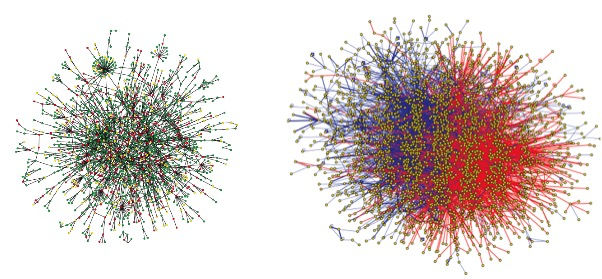
\includegraphics[scale=0.67]{interact}

\begin{small}\textit{\textbf{Figura 2.1}: Interattoma del lievito (sinistra) ed interattoma umano (destra)}.\end{small}
\end{center}

A questo punto, tuttavia, è necessario sottolineare i limiti dei dati PPI disponibili. La nostra attuale conoscenza dell'interattoma è purtroppo incompleta e rumorosa (\textit{noisy}). I metodi di rilevamento delle PPI hanno dei limiti per quanto riguarda il numero di interazioni veramente fisiologiche che possono essere rilevate e tutti i metodi per ora realizzati ed implementati trovano sia falsi positivi che negativi.

\section{Proprietà delle PPIN}
In questa sezione diamo uno sguardo ad alcune delle proprietà più importanti delle PPIN.

\subsection{\textit{Effetto del piccolo mondo}}
Le \textit{reti di interazione proteina-proteina} sono soggette all'\textit{effetto del piccolo mondo}\footnote{L'effetto del mondo piccolo è una teoria che sostiene che tutte le reti complesse presenti in natura sono tali che due nodi qualsiasi possono essere collegati da un percorso costituito da un numero relativamente piccolo di collegamenti.}; ciò significa che intercorre una grande connettività tra le proteine (\textit{\textbf{Figura 3.1}}). In altre parole, si può dire che il \textit{diametro} della rete (il numero massimo di passi che separano due nodi qualsiasi) è piccolo, non importa quanto grande sia la rete. Questo, di solito, significa che i due nodi sono separati da meno di sei passi, in genere, che riflettono l'ormai ampiamente diffusa teoria dei \textit{sei gradi di separazione} usata nelle scienze sociali.

\begin{center}
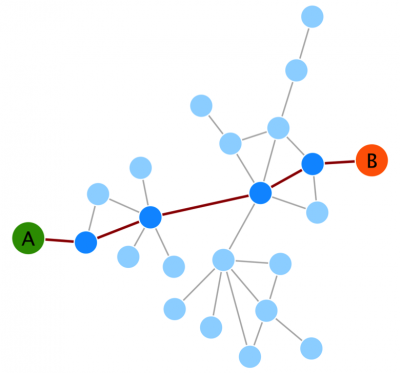
\includegraphics[scale=0.5]{grafo}

\begin{small}\textit{\textbf{Figura 3.1}: Effetto del piccolo mondo}.\end{small}
\end{center}

Questo livello di connettività ha importanti conseguenze biologiche, poiché consente un flusso efficiente e rapido dei segnali all'interno della rete stessa. 

A questo punto sorge spontanea una domanda: \textit{se la rete è così strettamente connessa, perché le perturbazioni in un singolo gene o in una singola proteina non hanno conseguenze drammatiche per la rete?} I sistemi biologici sono estremamente robusti e possono far fronte a una quantità relativamente elevata di perturbazioni in singoli/e geni/proteine. Per spiegare come ciò possa accadere, dobbiamo considerare un'altra proprietà fondamentale delle PPIN, che vedremo nella prossima sottosezione.

\subsection{\textit{Scale-free networks}}
Le \textit{reti di interazione proteina-proteina} sono \textit{\textbf{scale-free networks}}. La maggior parte dei nodi (che corrispondono alle proteine) nelle \textit{scale-free networks} hanno solo poche connessioni con altri nodi, mentre altri (denominati \textit{hub}) sono collegati a molti altri nodi della rete stessa (\textit{\textbf{Figura 3.2}}).

\begin{center}
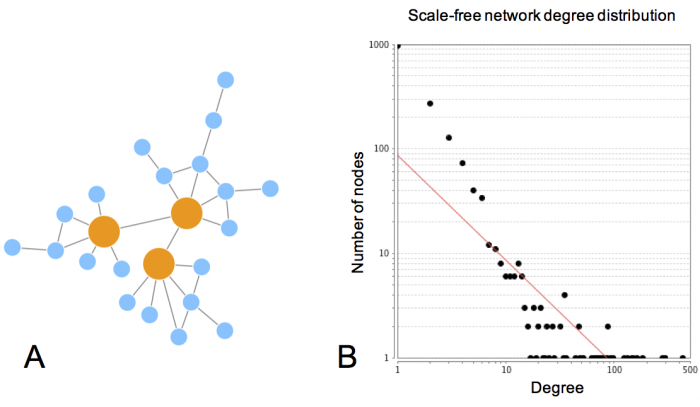
\includegraphics[scale=0.5]{graffo}

\begin{small}\textit{\textbf{Figura 3.2}: Il numero di connessioni di ogni nodo è chiamato \textbf{grado}. Se rappresentiamo la distribuzione del grado di una \textit{scale-free network} in scala logaritmica, possiamo vedere come si adatta ad una linea, avendo un piccolo numero di nodi con un alto grado (gli hub) e un grande numero di nodi con un basso grado.}.\end{small}
\end{center}

Le \textit{scale-free networks} possono essere costruite seguendo il modello di collegamento preferenziale, noto anche come il principio "\textit{rich get richer}". Questo principio afferma semplicemente che le \textit{scale-free networks} possono essere costruite aggiungendo archi che sono preferibilmente collegati a quei nodi con un grado più elevato.

La natura \textit{scale-free} delle \textit{reti di interazione proteina-proteina} conferisce loro una serie di importanti caratteristiche:
\begin{enumerate}
\setlength{\itemsep}{1pt}
  \setlength{\parskip}{0pt}
  \setlength{\parsep}{0pt}
\item \textbf{Stabilità}
\begin{itemize}
\setlength{\itemsep}{1pt}
  \setlength{\parskip}{0pt}
  \setlength{\parsep}{0pt}
\item Se i guasti si verificano in modo casuale e la maggioranza delle proteine costituisce un grado di connettività basso, la probabilità che un \textit{hub} venga colpito è minima.
\item Se si verifica un \textit{hub-failure}, la rete generalmente non perde la sua connettività grazie ai restanti \textit{hub}.
\end{itemize}

\item \textbf{Invarianza ai cambiamenti di scala}
\begin{itemize}
\item Non importa quanti nodi o archi abbia la rete, le sue proprietà rimangono stabili.
\item La presenza di nodi è ciò che consente l'\textit{effetto piccolo mondo} indipendentemente dalle dimensioni della rete.
\end{itemize}

\item \textbf{Vulnerabilità agli attacchi mirati}
\begin{itemize}
\item Se si perdono alcuni \textit{hub} principali, la rete si trasforma in un insieme di grafi isolati.
\end{itemize}
\end{enumerate}

\subsection{Transitività}
Un'altra caratteristica cruciale delle PPIN è la loro modularità. La \textit{\textbf{transitività}} o \textit{coefficiente di clustering} di una rete misura la tendenza dei nodi a raggrupparsi. Un'alta transitività significa che la rete contiene "comunità" o gruppi di nodi che sono densamente connessi (seguendo un'analogia delle scienze sociali, "gli amici dei miei amici sono miei amici"). Nelle reti biologiche, trovare queste comunità è molto importante perché possono aiutare ad individuare  \textbf{complessi proteici} (a titolo di esempio si veda la \textit{\textbf{Figura 3.3}}).

\begin{center}
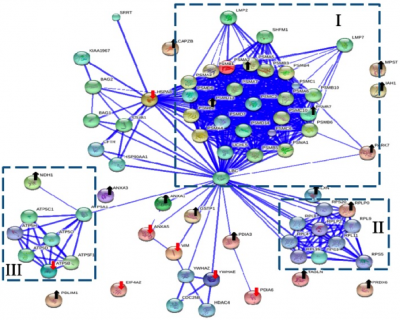
\includegraphics[scale=0.7]{grafffo}

\begin{small}\textit{\textbf{Figura 3.3}: Cluster topologici che riflettono la funzione biologica. I cluster sono evidenziati all'interno di quadrati a linee tratteggiate}.\end{small}
\end{center}

I \textit{complessi proteici} possono essere considerati un tipo di \textit{\textbf{modulo}}\footnote{Un \textit{modulo} un componente di un più vasto sistema, che opera in quel sistema indipendentemente dalle operazioni di altri componenti} (un'unità funzionale ed intercambiabile) in cui le proteine interagiscono in modo stabile, mantenendo una configurazione più o meno costante sia nel tempo che nello spazio.

Lo studio dei moduli è utile anche per definire le \textit{interazioni intermodulari} tra le proteine.

\section{Sorgenti di dati, valutazione dell'affidabilità e misurazione della confidenza}
Il primo passo per eseguire l'analisi delle PPIN è, naturalmente, la costruzione di una rete. Ci sono diverse fonti di dati PPI che possono essere utilizzate ed è importante essere consapevoli dei loro vantaggi e svantaggi.

Essenzialmente, è possibile ottenere i dati PPI da:
\begin{enumerate}
\setlength{\itemsep}{1pt}
  \setlength{\parskip}{0pt}
  \setlength{\parsep}{0pt}
\item \textbf{Il proprio lavoro sperimentale}, dove si può scegliere come i dati sono rappresentati e memorizzati.
\item \textbf{Un database primario di PPI}. Questi database estraggono le PPI dalle prove sperimentali riportate in letteratura utilizzando un processo di cura manuale. Sono i principali fornitori di dati PPI.
\item \textbf{Un database di metadati o un database predittivo}. Queste risorse riuniscono le informazioni fornite da diversi database primari e forniscono all'utente una rappresentazione unificata dei dati. 
I database predittivi vanno oltre e utilizzano i set di dati prodotti in modo sperimentale per prevedere, dal punto di vista puramente computazionale, le interazioni in aree inesplorate dell'interattoma. Questi dataset, tuttavia, sono in genere più "rumorosi" di quelli provenienti da altre fonti.
\end{enumerate}

Spesso sarà necessario integrare dati PPI provenienti da più fonti, poiché nessun database ha una rappresentazione completa di tutte le informazioni necessarie. Ciò crea alcune sfide interessanti, poiché diversi database utilizzano  identificatori diversi e contengono diversi tipi di dati.\\

A questo punto sorge, naturalmente, una preoccupazione che ha a che fare con l'analisi della rete: \textit{ci si può "fidare" del fatto che la rete di interazione rappresenti una "reale" interazione biologica?} Dato il rumore (\textit{noise}) insito nelle informazioni dell'interattoma, è importante essere rigorosi e attenti quando si valutano i dati delle \textit{interazioni proteina-proteina} che si utilizzano (potremmo trovarci di fronte a rindondanze ed incoerenze). È molto importante tener conto del fatto che la copertura dell'interattoma è incompleta e frammentaria, per questo motivo esistono molti metodi diversi per accertare l'affidabilità dei dati che si stanno considerando. Alcune strategie si avvalgono dei seguenti metodi:
\begin{enumerate}
\item \textbf{Informazioni biologiche contestuali} riguardanti le proteine e/o le molecole che sono coinvolte nell'interazione.
\item \textbf{Contare quante volte una data interazione è stata riportata in letteratura}. Questo è un approccio molto popolare e semplice; esistono varianti più elaborate di questa strategia, come il metodo MIscore\footnote{Per una descrizione completa e rigorosa di questo metodo rimandiamo alla lettura del seguente paper (non inserito nella \textbf{Bibliografia} alla fine di questo documento): Villaveces, J.M., et al., Merging and scoring molecular interactions utilising existing community standards: tools, use-cases and a case study. Database (Oxford), 2015. 2015. }.
\item \textbf{Metodi aggregati} che utilizzano una serie di strategie diverse e le integrano in un unico punteggio, come INTscore\footnote{A titolo informativo, il paper (non inserito nella \textbf{Bibliografia} alla fine di questo documento) riguardante l'INTscore è il seguente: Kamburov, A., Stelzl, U., and Herwig, R. IntScore: a web tool for confidence scoring of biological interactions. Nucleic Acids Res, 2012. 40(Web Server issue): p. W140-6.}.
\end{enumerate}

\pagebreak
\section{Analisi topologica delle PPIN}
L'analisi delle caratteristiche topologiche di una rete è un modo utile per identificare i partecipanti e le sottostrutture rilevanti che possono avere un significato biologico. Ci sono molte strategie diverse che possono essere usate per fare questo (si veda la \textit{\textbf{Figura 5.1}}). 

In questa sezione ci concentriamo sull'analisi della centralità (\textit{centrality analysis}) e sul clustering topologico (\textit{topological clustering}).

\begin{center}
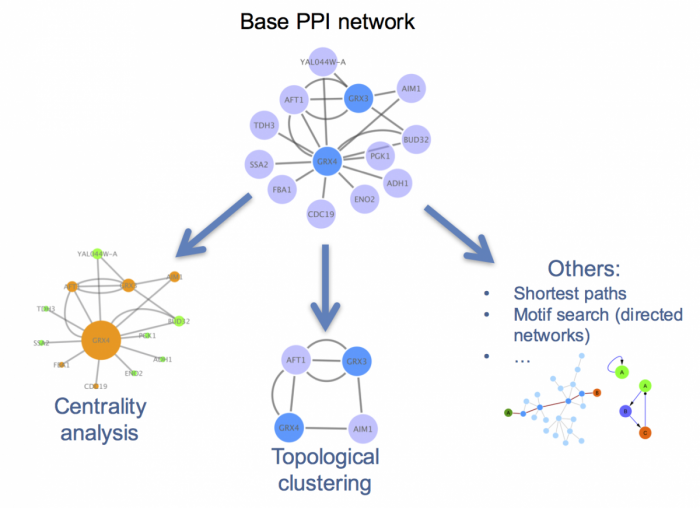
\includegraphics[scale=0.43]{ppin}

\begin{small}\textit{\textbf{Figura 5.1}: Strategie comuni di analisi strutturale per i PPIN}.\end{small}
\end{center}

\subsection{\textit{Centrality Analysis}}
La \textit{centralità} fornisce una stima di quanto sia importante un nodo o un arco per la connettività della rete (\textit{\textbf{Figura 5.2}}).
L'analisi della centralità nelle PPIN di solito mira a rispondere alla seguente domanda: \textit{quale proteina è la più importante e perché?}

\begin{center}
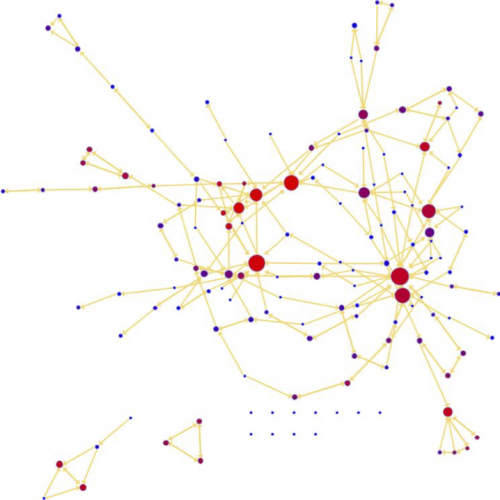
\includegraphics[scale=0.4]{ca}

\begin{small}\textit{\textbf{Figura 5.2}: Centralità del nodo rappresentato in una rete. I nodi più grandi e più rossi hanno valori di centralità più alti in questa rappresentazione. }.\end{small}
\end{center}

La definizione di \textit{centralità} varia a seconda del contesto o dello scopo dell'analisi che si sta eseguendo e può essere misurata utilizzando diverse metriche e criteri, per esempio:

\begin{enumerate}
\setlength{\itemsep}{1pt}
  \setlength{\parskip}{0pt}
  \setlength{\parsep}{0pt}
\item Il \textbf{grado dei nodi}.
\item Le \textbf{misure di centralità globale}. Due delle misure di centralità globale più utilizzate sono le centralità di \textit{prossimità} (\textit{closeness centrality}) e di \textit{interrelazione} (\textit{betweenness centrality}).

La \textit{closeness centrality} è una misura che stima la velocità del flusso di informazioni attraverso un dato nodo verso altri nodi. Essa misura quanto sono brevi i percorsi da un nodo verso tutti gli altri nodi.

La \textit{betweenness centrality} misura la frequenza con cui un nodo viene a trovarsi su tutti i percorsi più brevi fra due nodi\footnote{Questi nodi possono rappresentare proteine importanti nei percorsi di segnalazione e possono formare obiettivi per la scoperta di farmaci. Combinando questi dati con l'analisi delle interferenze possiamo simulare attacchi mirati alle PPIN e prevedere quali proteine sono candidati migliori per la ricerca di farmaci.}.
\end{enumerate}

\subsection{\textit{Clustering Analysis}}
La ricerca di "comunità" all'interno di una rete è una buona strategia utile a ridurre la complessità della rete stessa e ad estrarre moduli funzionali (ad esempio, complessi proteici). I \textit{\textbf{cluster}} sono un gruppo di nodi che sono più connessi al loro interno che con il resto della rete. Quando si parla di PPIN, le comunità rientrano in due categorie: moduli funzionali e complessi proteici (si veda la \textit{\textbf{Sottosezione 3.3}} per la corretta definizione dei termini).

\subsubsection{Metodi di \textit{Clustering Analysis}}
Ora presentiamo brevemente due metodi che utilizzano esclusivamente la topologia della rete per individuare componenti strettamente connesse tra loro. Bisogna sottolineare che non si fanno ipotesi sulla struttura interna dei \textit{cluster}, concentreremo pertanto la nostra attenzione soltanto sulle regioni ad alta densità.

\begin{center}
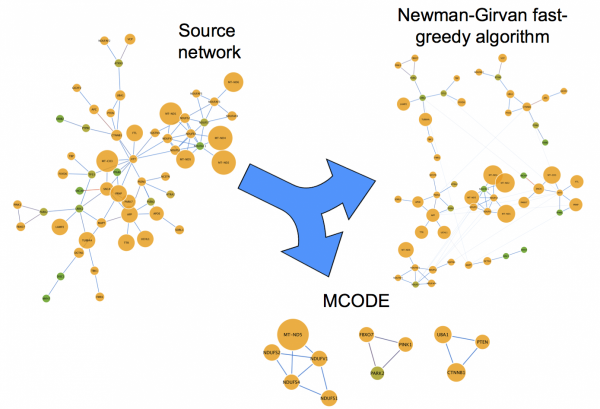
\includegraphics[scale=0.6]{ng}

\begin{small}\textit{\textbf{Figura 5.3}: Metodi di Clustering Analysis}.\end{small}
\end{center}

È importante notare che trovare la migliore struttura di comunità è algoritmicamente complesso ed è possibile solo per reti molto piccole. Per questo motivo sono stati sviluppati molti metodi di approssimazione.
\begin{enumerate}
\item \textbf{Algoritmo \textit{Newman-Girvan fast-greedy}}: Questo metodo "naïve" identifica i \textit{cluster} utilizzando la \textit{edge betweenness centrality measure}. Gli archi che collegano i diversi \textit{cluster} hanno \textit{centrality values} più elevate. Per definire i \textit{cluster} il metodo utilizza \textit{edge betweenness centrality scores} per classificare gli archi della rete, quindi rimuove gli archi più centrali e ricalcola i \textit{betweenness scores} fino a quando non rimangono più archi. Gli archi interessati dalla rimozione sono considerati parte dello stesso \textit{cluster}.
\item \textit{\textbf{Algoritmo MCODE}}: Questo metodo è stato appositamente sviluppato per trovare complessi proteici nelle PPIN. Più rigoroso dell'algoritmo Newman-Girvan, mira a trovare solo quelle sottoreti che sono altamente interconnesse (rappresentanti complessi proteici relativamente stabili, che funzionano come una singola entità nel tempo e nello spazio).
L'algoritmo utilizza un processo a tre fasi: (1) con il \textit{weighting} un punteggio più alto viene dato a quei nodi i cui vicini sono più interconnessi; (2) partendo dal nodo (denominato \textit{seed}) con il peso più elevato, vengono aggiunti al complesso i nodi che hanno un peso superiore ad una determinata soglia; (3) infine vengono applicati dei filtri per migliorare la qualità del \textit{cluster}.
\end{enumerate}

\section{PPIN: \textit{Annotation enrichment analysis}}
Ci sono molti approcci diversi che possono essere utilizzati per comprendere il contesto biologico delle PPIN. L'\textit{Annotation enrichment analysis} è uno dei metodi più popolari. Anche se non è propriamente uno strumento di analisi delle reti, è spesso utilizzato in combinazione con l'analisi topologica delle reti.

Si utilizzano le annotazioni geniche/proteine fornite, per esempio, dall'Ontologia Genica (GO) per rispondere, tramite un test statistico, alla seguente domanda:
\begin{center}
"Quando si campionano $X$ proteine (\textit{test set}) da $N$ proteine (\textit{reference set}; grafo o \textit{annotation}), qual è la probabilità che $x$, o più, di queste proteine appartengano ad una categoria funzionale $C$ condivisa da $n$ delle $N$ proteine nel \textit{reference set}?"
\end{center}
Il risultato di questo test ci fornisce una lista di termini che descrivono la rete (o una parte di essa) nel suo insieme, per identificare le "comunità" interconnesse trovate attraverso il \textit{topological clustering}.

I principali limiti dell'\textit{Annotation enrichment analysis} derivano dalle \textit{annotation} stesse. Alcune aree della biologia sono annotate più approfonditamente e meglio descritte di altre, con termini più dettagliati e più precisi (nel nostro caso, solo le proteine più "popolari" sono meglio annotate). Questo introduce una certa "distorsione" nell'analisi statistica.

È anche importante notare che i termini nell'Ontologia Genica (GO) possono essere assegnati sia da un curatore umano che esegue un'attenta annotazione manuale, sia da approcci computazionali che utilizzano le basi dell'annotazione manuale per dedurre quali termini descriverebbero in modo corretto i prodotti genici non scoperti. Ne consegue che un'altra limitazione è costituita dalla complessità e dal dettaglio dell'annotazione associati a grandi insiemi di geni/proteine. 

\pagebreak
\section{MTGO}
Il metodo MTGO - \textit{Module detection via Topological information and GO knowledge} - costituisce un nuovo approccio di identificazione dei moduli funzionali nelle PPIN. Questo metodo combina le informazioni provenienti dalla topologia delle reti con la conoscenza biologica relativa alle proteine.
 
Per identificare i moduli più interessanti, MTGO utilizza partizioni ripetute della rete sfruttando la \textit{modularità} del grafo (= funzione che misura la qualità topologica di una determinata partizione in un grafo). La partizione viene successivamente appresa attraverso un processo di ottimizzazione che tiene conto della struttura della rete e della sua natura biologica. A differenza dei precedenti approcci basati su GO, MTGO fornisce un unico termine GO che descrive al meglio la natura biologica di ogni modulo identificato.

Evidenziando i principali processi coinvolti nel sistema biologico, rappresentato dai modelli di PPIN, e grazie al suo modo unico di sfruttare l'Ontologia Genica, MTGO si differenzia in maniera significativa dagli algoritmi allo stato dell'arte (ClusterOne, MCODE, COACH, CFinder, Markov Cluster -MCL-, DCAFP e GMFTP). 
%Le prestazioni di tali metodi sono state valutate sia da una prospettiva a livello di rete, sia con un'analisi relativa al rilevamento di moduli sparsi e/o di piccola dimensione.

Per valutare le performance di MTGO sono state selezionate, per i test, quattro PPIN reali: Krogan, Gavin, Collins e DIP Hsapi PPIN.

\begin{center}
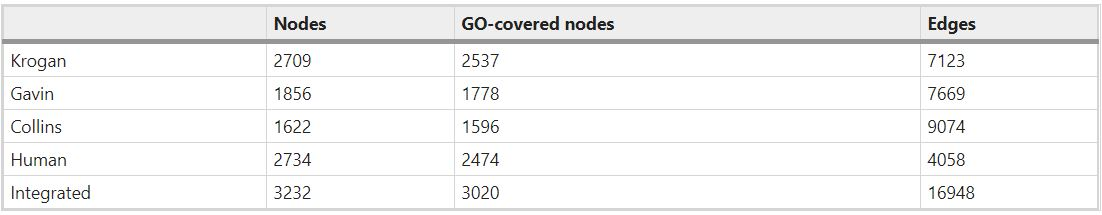
\includegraphics[scale=0.53]{tab1}

\begin{small}\textit{\textbf{Figura 7.1}: In questa tabella vengono indicate le caratteristiche principali di ogni rete, incluso il numero di nodi coperti dai termini GO, usati come input per MTGO}.\end{small}
\end{center}

I termini GO utilizzati come input per MTGO includono le seguenti tre categorie: \textit{Componente Cellulare}, \textit{Processo Biologico} e \textit{Funzione Molecolare}. 
MTGO ha mostrato i risultati migliori otto volte su nove ed è in grado di individuare complessi piccoli/sparsi anche in reti molto grandi.

MTGO è in grado di individuare moduli funzionali all'interno delle PPIN, prevede l'\textit{overlapping} e la copertura totale della rete\footnote{Si definisce \textit{copertura di nodi} (\textit{vertex cover}) di un grafo un insieme $C$ di nodi con la proprietà che ogni arco nel grafo abbia almeno uno dei suoi estremi in $C$.}, due \textit{features} importantissime per gli algoritmi di identificazione di moduli.

MTGO prevede una mappa sia dei moduli topologici che funzionali. I moduli topologici assicurano la copertura totale della rete, mentre quelli funzionali condividono i nodi, permettendo l'\textit{overlapping}; il metodo dipende fortemente dalla qualità dei termini GO (le sue performance infatti diminuiscono significativamente a seconda della perturbazione, del 25\%, 50\% e 75\%, dei termini GO forniti) ed è stato progettato per essere testato sia su reti pesate che non. 

MTGO possiede l'abilità di individuare un insieme di termini GO fornendo un'interpretazione biologica significativa della PPIN, proprietà assente negli altri algoritmi allo stato dell'arte.\\

\subsection{Descrizione di MTGO}
Una PPIN può essere rappresentata tramite un grafo $G = (V,E)$ dove $V$ ed $E$ corrispondono ai nodi e agli archi della rete, rispettivamente. $V$ è l'insieme delle proteine ed è definito come $V =\left \{v_1, v_2, v_3, ..., v_N\right \}$ dove $N$ è il numero di proteine/nodi totale. $E$ rappresenta l'insieme delle relazioni tra i nodi della rete: $E = \left \{e_i,j\right \}$, $(i,j) \in$ [1,$N$]. Inoltre, $G$ detiene le proprietà topologiche PPI. Per integrare le informazioni relative alle funzioni biologiche all'interno della rete, ai nodi vengono associati i termini GO. MTGO calcola l'insieme $T = (L, \Delta)$, dove il $p$-esimo elemento è $t_p = (l_p, \delta_p)$, $l_p$ rappresenta l'\textit{ontology term}, mentre $\delta_p$ è l'$l_p$-insieme associato alla rete di proteine (si veda la \textit{\textbf{Figura 7.2}} per un esempio).

\begin{center}
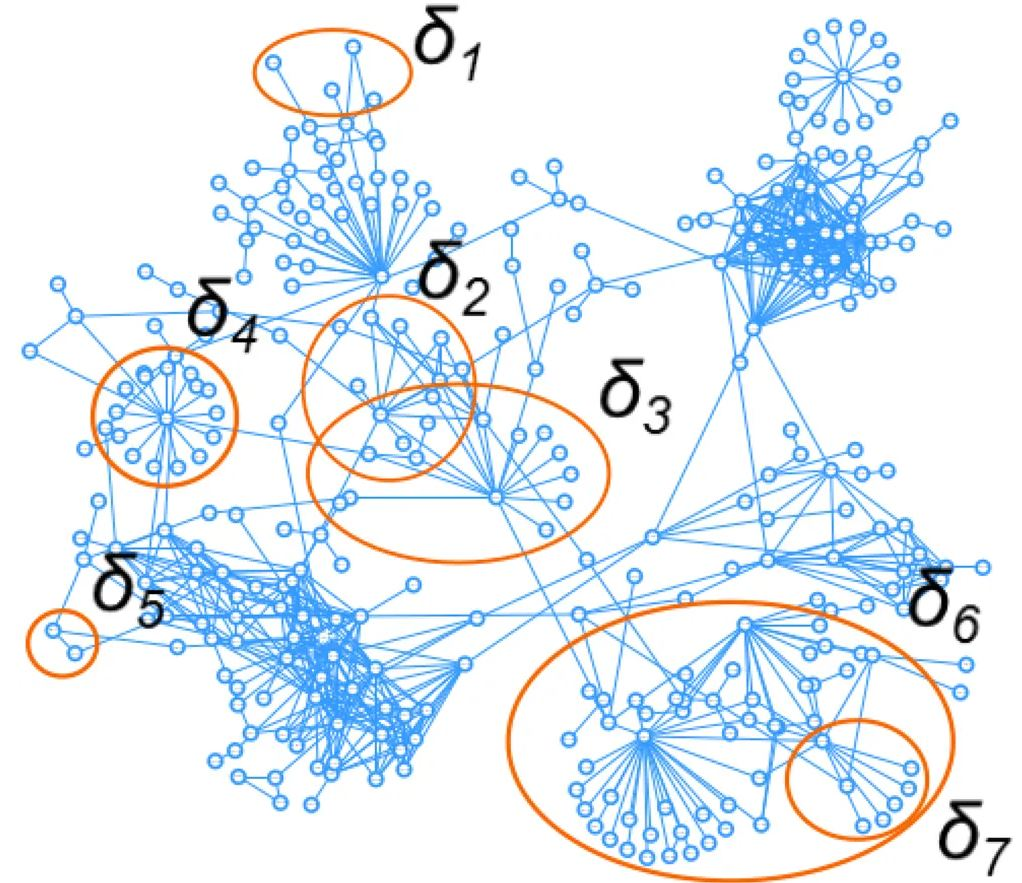
\includegraphics[scale=0.4]{delta}

\begin{small}\textit{\textbf{Figura 7.2}: Esempio dei $\delta$ elementi rappresentati in una rete, potrebbero condividere più nodi o essere inclusi in una categoria più vasta}.\end{small}
\end{center}

$I = (G,T)$ è l'input del sistema. L'obiettivo di MTGO è quello di processare $G$ per trovare gruppi di nodi che condividono sia le proprietà topologiche $(V,E)$, sia quelle funzionali $(T)$. L'output di questo metodo è $R^F = (C^F, \Phi^F)$ dove $C^F$ è l'insieme dei moduli topologici, mentre $\Phi^F$ è l'insieme dei moduli funzionali. Da notare che $|C^F| = |\Phi^F|$, la relazione è 1:1. 

MTGO calcola iterativamente $C$ e $\Phi$ e la coppia $R^F = (C^F, \Phi^F)$ viene selezionata come output finale.

L'insieme di moduli topologici $C$ costituisce una partizione della rete, $C = \left \{c_1, ..., c_h, ..., c_H\right \}$, di modo che:

\begin{center}
$c_1 \cap c_2 ... \cap c_h ... \cap c_H \equiv \emptyset$
\end{center}
\begin{center}
 $c_1 \cup c_2 ... \cup c_h ... \cup c_H \equiv V$
\end{center}

Bisogna notare che ogni nodo di una partizione di $C$ viene unicamente assegnata ad un singolo modulo topologico. D'altra parte, l'insieme $\Phi = \left \{\phi_1, ..., \phi_h, ..., \phi_H\right \}$ descrive i moduli funzionali coinvolti nella rete. $\Phi$ viene definito in questo modo:

\begin{center}
$\phi_1 \cap \phi_2 ... \cap \phi_h ... \cap \phi_H \equiv \emptyset$
\end{center}
\begin{center}
 $\phi_1 \cup \phi_2 ... \cup \phi_h ... \cup \phi_H \subseteq V$
\end{center}

e $\Phi \subset T$, cioè $\Phi$ è il sottoinsieme di $T$ selezionato da MTGO per descrivere le funzioni biologiche collegate alla partizione $C$ della PPIN.

La copertura completa (\textit{full coverage}) e la sovrapposizione (\textit{overlapping}) sono considerate le caratteristiche ideali degli algoritmi di identificazione di moduli. MTGO garantisce entrambe queste proprietà con il suo doppio output complementare $C$ e $\Phi$. In particolare, i moduli topologici $C$ rappresentano una partizione di rete, garantendo così una copertura completa per definizione. I moduli funzionali $\Phi$ si sovrappongono invece, consentendo l'assegnazione di un nodo a due o più moduli. Questa caratteristica è particolarmente importante in quanto riflette il comportamento dei sistemi biologici, dove una proteina può essere coinvolta in molteplici funzioni.

Vediamo ora di capire, per lo meno a livello intuitivo, i passi eseguiti da MTGO.
Dato l'input $I = (G,T)$, MTGO realizza tre fasi principali: (1) inizializzazione, (2) iterazione e (3) controllo della convergenza.

\begin{center}
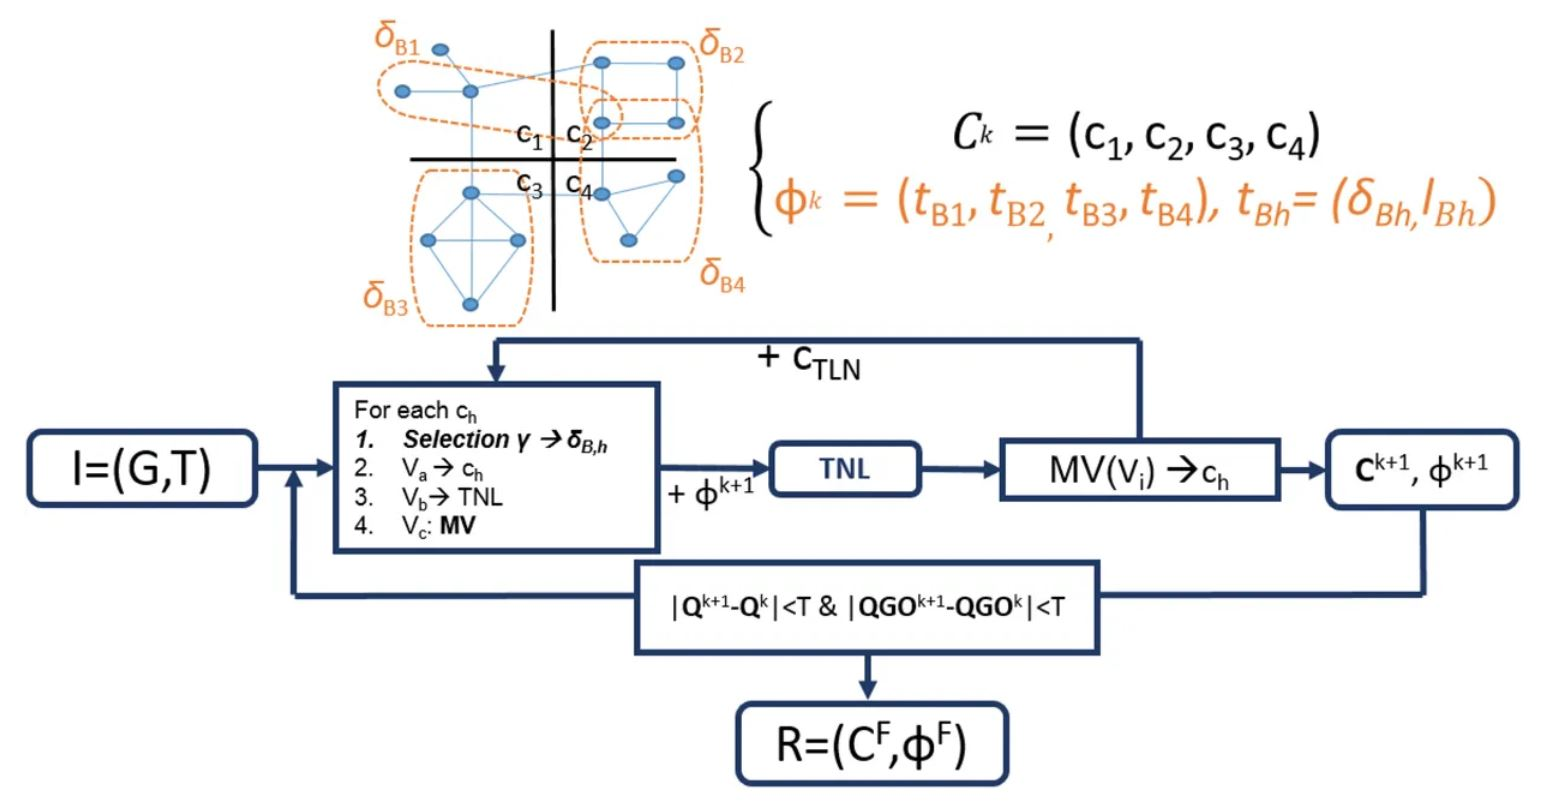
\includegraphics[scale=0.4]{algMTGO}

\begin{small}\textit{\textbf{Figura 7.3}: Rappresentazione dei passi seguiti dall'algoritmo MTGO}.\end{small}
\end{center}

\subsubsection{Inizializzazione}
Nella fase di inizializzazione, $V$ viene utilizzato per generare una partizione casuale $C^0$ (\textit{\textbf{Figura 7.4 A}}) nella quale il numero di moduli topologici è $\propto \sqrt{N}$. $T$ viene creato partendo da una \textit{GO term list} fornita dall'utente (in conformità all'insieme $V$). Vengono successivamente definiti, sempre dall'utente, due parametri ($minSize$ e $maxSize$) che definiscono la minima e la massima taglia dei moduli in $T$, cioè il numero di nodi in un $\delta_p$.

\begin{center}
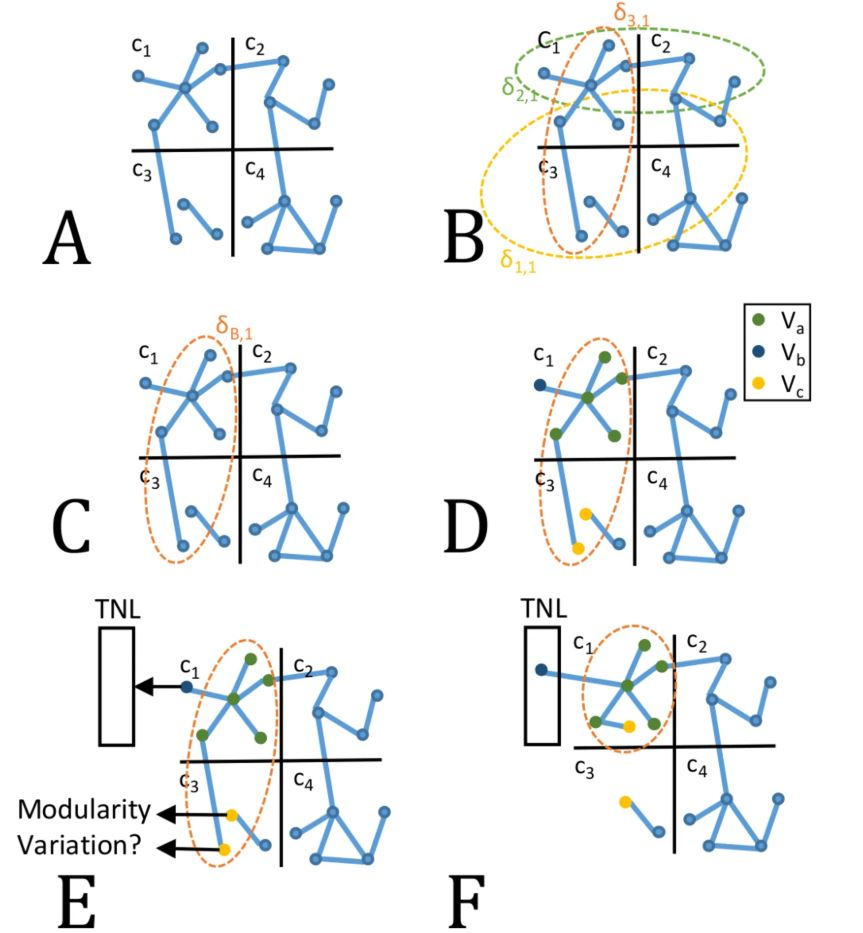
\includegraphics[scale=0.6]{MTGO2}

\begin{small}\textit{\textbf{Figura 7.4}: Le fasi di MTGO}.\end{small}
\end{center}

\subsubsection{Iterazione}
Ad ogni iterazione viene calcolata una coppia $(C, \Phi)$, in particolare $C$ ri-assegnando i nodi alla partizione precedente e $\Phi$ selezionando elementi da $T$ che descrivono al meglio $C$. Ogni partizione di $C$ è costituita da $c_h$ moduli topologici con $h$ rappresentante l'indice di una singolo modulo topologico ($1\leq h \leq H$, il numero totale dei moduli funzionali $H$ varia ad ogni iterazione). Idealmente, MTGO tende ad assegnare i nodi in modo che i moduli topologici coincidano con quelli funzionali\footnote{Per una trattazione dettagliata di questa fase rimandiamo alla lettura delle due sottofasi descritte nel dettaglio al seguente sito: https://www.nature.com/articles/s41598-018-23672-0Tab1}.

\begin{center}
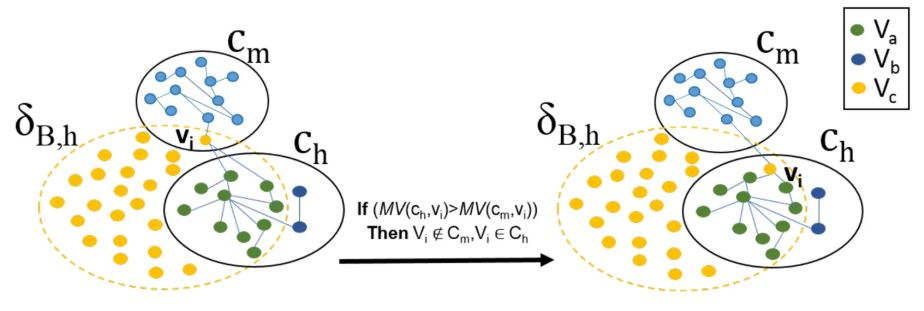
\includegraphics[scale=0.64]{deltaa}

\begin{small}\textit{\textbf{Figura 7.5}: Riassegnamento di un nodo}.\end{small}
\end{center}

\subsubsection{Convergenza}
Per valutare se la convergenza è stata raggiunta o meno si utilizzano due funzioni: \textit{modularità} ($Q$) e \textit{Quality GO} ($QGO$). $Q$ valuta la qualità globale della partizione $C$, mentre $QGO$ valuta la corrispondenza tra $C$ e $\Phi$. Idealmente, $C$ e $\Phi$ dovrebbero essere soggette ad \textit{overlapping}.

La formula di $Q$ è:

\begin{center}
$Q(C^k) = \displaystyle{\sum_{1<h<H_k}\frac{e^k_h}{|E|} - \left(\frac{d^k_h}{2 \times |E|}\right)^2}$
\end{center}

Questa formula serve a valutare le partizioni dei grafi. L'indice $k$ indica la $k$-esima iterazione dell'algoritmo. $C^k$ è la $k$-esima partizione, $H^k$ è il numero di moduli topologici. $e^k_h$ è il numero totale di archi nell'$h$-esimo modulo topologico mentre $d^k_h$ è la somma dei gradi dei nodi dell'$h$-esimo modulo topologico. 

Il valore di $Q$ varia da -1 a 1, i valori positivi (negativi) indicano un maggior (minor) numero di collegamenti all'interno dei moduli topologici rispetto ad una randomizzazione. 

\begin{center}
$QGO(C^k) = \frac{\displaystyle{\sum_{1<h<H_k}|\delta^k_{B,h} \cap c^k_h|}}{N_{GO}}$
\end{center}

Senza scendere troppo nei dettagli, a livello intuitivo, è sufficiente dire che la formula $QGO$ serve a valutare il grado di \textit{overlapping} tra $C^k$ e $\Phi^k$.

\pagebreak
\section{IsoRank}
IsoRank è un metodo per l'allineamento globale di più PPIN. L'intuizione da tener presente è che una proteina in una rete PPI costituisce una buona corrispondenza (\textit{match}) per una proteina in un'altra rete se le loro rispettive sequenze e i loro intorni topologici sono una buona corrispondenza. Utilizzando IsoRank, calcoliamo un allineamento globale delle reti PPI \textit{Saccharomyces cerevisiae}, \textit{Drosophila melanogaster}, \textit{Caenorhabditis elegans}, \textit{Mus musculus} e \textit{Homo sapiens} (i sottografi individuati con questi allineamenti sono più grandi e più vari di quelli prodotti dai metodi precedenti). Metodi precedenti hanno dimostrato la loro efficacia nell'identificare pattern localizzati confrontando tra di loro due reti. Questo metodo rappresenta un grande passo avanti per l'allineamento di più reti PPI ed è applicabile in molti settori scientifici.

IsoRank rappresenta un approccio di analisi comparativa delle reti PPI al fine di trovare una soluzione al problema di allineamento ottimo \textit{globale} tra due o più PPIN, mirando a trovare la corrispondenza tra i nodi e gli archi delle reti in input che massimizzi il \textit{match} totale tra le reti.

\subsection{Global vs. Local Network Alignment}
In generale, l'obiettivo in un problema di allineamento di rete è quello di trovare un sottografo comune (cioè un insieme di archi conservati) tra le reti in input. Corrispondentemente a questi archi conservati, esiste una mappatura tra i nodi delle reti. Per esempio, quando la proteina $a_1$ dalla rete $G_1$ viene mappata sulle proteine $a_2$ in $G_2$ e $a_3$ in $G_3$, allora $a_1$, $a_2$ e $a_3$ si riferiscono allo stesso nodo nell'insieme degli archi conservati. Ciò che rende difficile il problema è il compromesso (\textit{trade-off}) da ottenere: massimizzare la sovrapposizione (\textit{overlap}) tra le reti (cioè il numero di archi conservati), garantendo al tempo stesso che le proteine mappate siano il più possibile correlate.


L'obiettivo nel GNA è quello di trovare il miglior allineamento complessivo tra le reti in ingresso. Un algoritmo LNA è essenzialmente destinato a trovare motivi/pattern simili tra due reti; in GNA, tuttavia, l'obiettivo è quello di trovare un'unica mappatura coerente che copra tutti i nodi tra tutti i grafi in input. Inoltre, deve esserci \textit{transitività}: se $a_1$ in $G_1$ viene mappata su $a_2$ in $G_2$ e $a_2$ viene mappata su $a_3$ e $a_4$ in $G_3$, allora anche $a_1$ dovrebbe essere mappato su $a_3$ e $a_4$. Il GNA può essere usato per confrontare gli interattomi e per comprendere le variazioni tra specie.

\subsection{\textit{Score} e \textit{mapping}}
Consideriamo un semplice caso di GNA a coppie. L'input consiste in due PPIN $G_1$ e $G_2$. Ogni arco $e$ può aver associato un peso $w(e)$ ($0\leq w(e) \leq1$). Inoltre, l'input consiste anche di una \textit{similarity measure} tra i nodi delle due reti.

L'output desiderato è un mapping tra i nodi delle due reti che massimizza la combinazione convessa delle seguenti funzioni obiettivo: (1) la dimensione del grafo in comune in seguito al mapping e (2) la somiglianza tra le sequenze dei nodi.

L'algoritmo prevede due fasi. Nella prima fase associa un \textit{functional similarity score} ad ogni possibile match tra i nodi delle due reti. Sia $R_{ij}$ lo score per la coppia di proteine ($i,j$) dove $i$ proviene dalla rete $G_1$, mentre $j$ da $G_2$. La seconda fase costruisce la mappatura per il GNA estraendo un insieme di score elevati (in accordo con il vettore \textit{\textbf{R}}).
Per calcolare il \textit{functional similarity score} $R_{ij}$ consideriamo la coppia ($i,j$) un buon match se le sequenze di $i$ e di $j$ si allineano e i loro rispettivi "vicini" costituiscono a loro volta un buon match(scrivi bene). Bisogna quindi creare un insieme di vincoli e calcolare i \textit{neighborhood scores} in modo ricorsivo. Si consideri la seguente equazione:

\begin{center}
\textit{\textbf{R}} = $\sum R_{ij}$ = $\displaystyle{\sum_{u \in N(i)}} \displaystyle{\sum_{v \in N(j)}\frac{1}{|N(i)||N(j)|} R_{ij}}$ con $i \in V_1$, $j \in V_2$
\end{center}

$N(a)$ rappresenta tutti i \textit{neighbors} del nodo $a$; $|N(a)|$ la cardinalità di questo insieme; $V_1$ e $V_2$ sono gli insiemi dei nodi nelle reti $G_1$ e $G_2$ rispettivamente. Lo score $R_{ij}$ dipende dagli score dei vicini di $i$ e $j$, che a loro volta dipendono dai vicini dei vicini etc. I nodi che hanno una buona corrispondenza hanno valori score $R_{ij}$ più alti.

\begin{center}
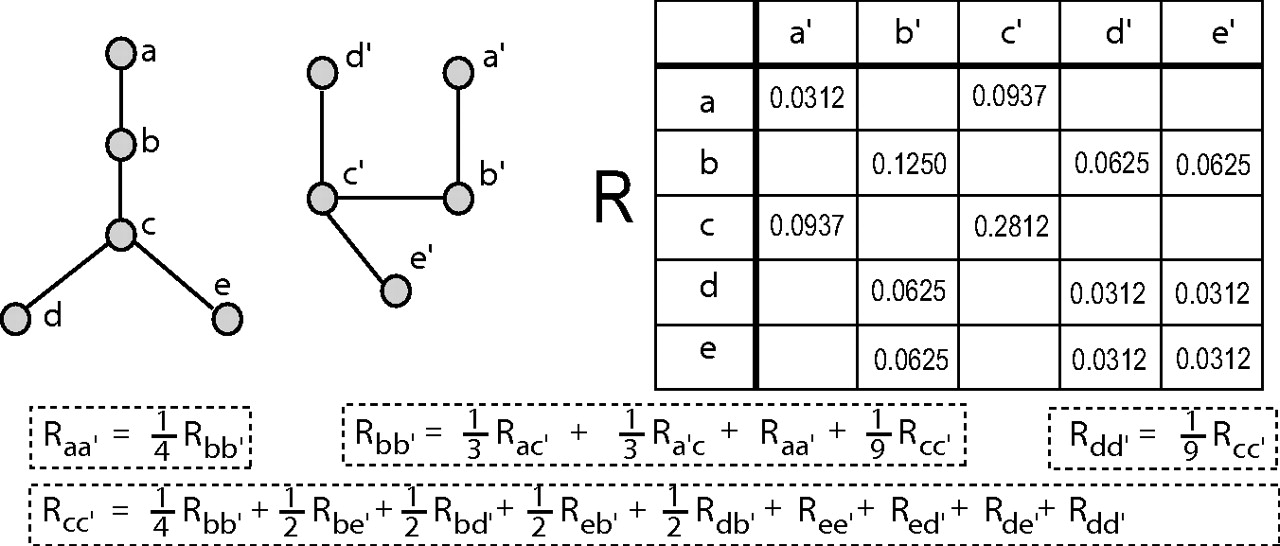
\includegraphics[scale=0.36]{isorank}

\begin{small}\textit{\textbf{Figura 8.1}: desc mancante vedi paper}.\end{small}
\end{center}

Multiple GNA
Quando l'input consiste di più di due reti, si ripete il processo appena descritto per tutte le possibili coppie di reti fornite in input e successivamente si calcolano i \textit{functional similarity scores} \textit{\textbf{R}} per ogni coppia di reti in input.

A questo punto dell'algoritmo abbiamo uno score $R_{ij}$ per ogni coppia di nodi che non sono nella stessa rete; in genere, per il 99\% delle coppie-nodo, questo valore è zero. Dopo aver identificato gli score più alti bisogna assicurarsi che il mapping mantenga la propietà di transitività (descritta in precedenza). Il mapping si può ottenere in due modi: 
\begin{enumerate}
\setlength{\itemsep}{1pt}
  \setlength{\parskip}{0pt}
  \setlength{\parsep}{0pt}
\item \textbf{One-to-one Mapping}: ogni nodo viene mappato in al massimo un altro nodo (per specie);
\item \textbf{Many-to-many}: un nodo può essere mappato in più di un nodo in un'altra specie.
\end{enumerate}

global alignment of yeast, fly, worm, human, and mouse networks

Il sottografo comune corrispondente all'allineamento globale possiede 1663 archi in comune ad almeno due PPIN e 157 archi in comune al almeno 3 PPIN. La dimensione dei sottografi comuni è relativamente piccola (solo $\approx$ 5\% della PPIN umana). Un motivo per il piccolo overlap tra le reti PPI potrebbe essere che (aaah riscrivi) i dati relativi sono incompleti o rumorosi. All'aumentare della quantità e della qualità dei dati, l'overlap dovrebbe aumentare sensibilmente. Delle 86932 proteine provenienti dalle 5 specie, 59539 (68,5\%) hanno ottenuto almeno un match in un'altra proteina di una rete diversa.


BLABLA
IsoRank mira a massimizzare la corrispondenza complessiva tra le due reti. Si basa sulla teoria dei grafici spettrali per calcolare i punteggi di allineamento di coppie di nodi di reti diverse; lo fa utilizzando l'euristico che due nodi sono una buona corrispondenza se anche i loro rispettivi vicini corrispondono bene. Così, il punteggio di una coppia di proteine dipende dal punteggio dei loro vicini, che, a loro volta, dipendono dai vicini dei loro vicini, e così via.
Una volta che questi punteggi 'topologici' sono calcolati per tutte le coppie di nodi, i punteggi BLAST basati sulla sequenza sono inclusi nei punteggi di allineamento a coppie. IsoRank costruisce quindi l'allineamento dei nodi con la strategia avida e ripetitiva di identificare tra tutte le coppie di proteine la coppia con il punteggio più alto, producendo quella coppia e rimuovendo tutti i punteggi che coinvolgono uno qualsiasi dei due nodi identificati.


\pagebreak
\section{Struc2vec}
Struc2vec è un framework flessibile per l'apprendimento di rappresentazioni latenti per l'identità strutturale dei nodi.
Utilizza una gerarchia per misurare la somiglianza dei nodi in scale diverse e costruisce un grafo multilivello per codificare le somiglianze strutturali e generare il contesto strutturale per i nodi.

L'identità strutturale è un concetto di simmetria in cui i nodi della rete vengono identificati in base alla struttura della rete e alla loro relazione con altri nodi.

Struc2vec presenta prestazioni molto elevate nell'acquisizione di nozioni di identità strutturale in quanto supera i limiti degli approcci precedenti.
Gli esperimenti numerici indicano che struc2vec migliora le prestazioni sulle attività di classificazione che dipendono maggiormente dall'identità strutturale.
Struc2vec eccelle anche quando la rete originale è soggetta a forti rumori casuali (rimozione casuale degli archi nel grafo).

In quasi tutte le reti, i nodi tendono ad avere una o più funzioni che determinano il loro ruolo nel sistema. Ad esempio, le proteine in una rete di interazione proteina-proteina (PPI) esercitano funzioni specifiche. 
Intuitivamente, diversi nodi in tali reti possono eseguire funzioni simili, come catalizzatori nella rete PPI di una cella. Pertanto, i nodi possono spesso essere partizionati in classi equivalenti rispetto alla loro funzione nella rete.

Le idee chiave di struc2vec sono:
\begin{itemize}
  \item Valutare la somiglianza strutturale tra i nodi indipendentemente dai loro attributi e quelli dei bordi, nonché la loro posizione nella rete.
Così, due nodi che hanno una struttura locale simile saranno considerati così, indipendentemente dalla posizione di rete e le etichette dei nodi nei loro quartieri.
Questo approccio inoltre non richiede un grafo connesso, identifica nodi strutturalmente simili anche in componenti connesse diverse.
  \item Stabilire una gerarchia per misurare la somiglianza strutturale, consentendo nozioni progressivamente più rigorose di ciò che significa essere strutturalmente simili.
In particolare, nella parte inferiore della gerarchia, la somiglianza strutturale tra i nodi dipende solo dai loro gradi, mentre nella parte superiore della gerarchia dipende dall'intera rete (dal punto di vista del nodo).
  \item Generare contesti casuali per i nodi (vettori), che sono sequenze di nodi strutturalmente simili come osservato da un camminato casuale pesato che attraversa un grafo multistrato (e non la rete originale). 
Pertanto, due nodi che appaiono frequentemente con contesti simili avranno probabilmente una struttura simile.
\end{itemize}

Considerando il problema delle rappresentazioni di apprendimento che catturano l'identità strutturale dei nodi nella rete. Un approccio corretto dovrebbe presentare due proprietà:
\begin{itemize}
  \item La distanza tra la rappresentazione latente dei nodi deve essere fortemente correlata alla loro somiglianza strutturale. Quindi, due nodi con strutture di rete locale identiche devono avere la stessa rappresentazione latente, mentre i nodi con identità strutturali diverse devono essere distanti.
  \item La rappresentazione latente non deve dipendere da alcun attributo del nodo o degli archi, incluse le etichette dei nodi.
Pertanto, i nodi strutturalmente simili devono avere una rappresentazione latente stretta, indipendente dagli attributi del nodo e dei lati nel proprio vicinato.
L'identità strutturale dei nodi deve essere indipendente dalla sua "posizione" nella rete.
\end{itemize}

Struct2vec è quindi un framework generale per l'apprendimento di rappresentazioni latenti per i nodi, composto da quattro passaggi principali:
\begin{itemize}
  \item Determinare la somiglianza strutturale tra ogni coppia di vertici nel grafo per dimensioni di vicinato diverse.
Ciò induce una gerarchia che fornisce maggiori informazioni per valutare la somiglianza strutturale a ogni livello della gerarchia.
  \item Costruire un grafo multilivello pesato in cui tutti i nodi della rete sono presenti in ogni livello e ogni livello corrisponde a un livello della gerarchia nella misurazione della somiglianza strutturale.
Inoltre, i pesi degli archi tra ogni coppia di nodi all'interno di ogni strato sono inversamente proporzionali alla loro somiglianza strutturale.
  \item Utilizzare il grafo multilivello per generare il contesto (un vettore) per ogni nodo.
In particolare, un cammino casuale sul grafo multilivello viene utilizzato per generare sequenze di nodi. 
È probabile che queste sequenze includano nodi che sono più strutturalmente simili.
  \item Applica una tecnica per imparare la rappresentazione latente da un contesto dato dalla sequenza di nodi, ad esempio Skip-Gram.
\end{itemize}

\subsection{Misurare la somiglianza strutturale}
Sia $G=(V,E)$ un grafo indiretto, non pesato, dove $n=|V|$ e $k^*$ il suo diametro.
Sia $R_k(u)$ l'insieme di nodi a distanza $k>=0$ da $u\in G$. In particolare, $R_1(u)$ rappresenta l'insieme dei vicini di $u$ ed in generale, $R_k(u)$ è l'anello di nodi a distanza $k$.
Sia $s(S)$ la sequenza di gradi ordinati di un insieme di nodi $S\subset V$.
Confrontando le sequenze di gradi ordinate degli anelli al distanza $k$ da $u$ e $v$ possiamo imporre una gerarchia per misurare la somiglianza strutturale di un insieme di nodi $S\subset V$.
In particolare, sia $f_k(u,v)$ la \textit{distanza strutturale} tra $u$ e $v$ quando si considera l'anello di nodi a distanza $k$.

--------EQUAZIONE 1 $f_k(u,v)=...$------------
dove $g(D_1,D_2)>=0$ misura la distanza tra le sequenze di gradi ordinati $D_1$ e $D_2$ e $f_{-1}=0$.

Se gli anelli di nodi a distanza $k$ di $u$ e $v$ sono isomorfi, e mappano $u$ in $v$, allora $f_{k-1}(u,v)$.

Lo step finale consiste nel determinare la funzione che confronta due sequenze di gradi ordinati.
Per realizzare ciò, viene adottata la Deformazione temporale dinamica (Dynamic Time Warping (DTW)) che trova l'ottimo allineamento tra due sequenze $A$ e $B$. In particolare, data una funzione di distanza $d(a,b)$ per gli elementi della sequenza, DTW accoppia ogni elemento $a\in A$ ad $b\in B$, in modo che la somma delle distanze tra gli elementi accoppiati è minima. Dato che gli elementi delle sequenze di $A$ e $B$ sono gradi di nodi, viene usata la seguente funzione di distanza:
--------EQUAZIONE 2 $d(a,b)=...$ ------------

Si noti che se $a=b$ allora $d(a,b)=0$. Quindi due liste uguali avranno distanza nulla.
Infine, mentre viene utilizzato DTW per valutare la somiglianza tra due sequenze di gradi ordinate, qualsiasi altra funzione di costo potrebbe essere adottata in questo framework.

\subsection{Costruzione del Grafo di contesto}
Costruiamo un grafo pesato multilivello che codifica la somiglianza strutturale tra nodi.
Sia $M$ il grafo multilivello dove il layer $k$ è definito usando l'anello di nodi a distanza $k$.
Ogni livello $k=0,...,k^*$ è formato da un grafo completo, pesato, non diretto con l'insieme di nodi $V$ e quindi $\binom{n}{2}$ archi. Il peso dell'arco ttra due nodi in un livello è dato da:
--------EQUAZIONE 3 $w_k(u,v)=...$ ------------
Si noti che gli archi sono definiti solo se $f_k(u,v)$ è definito e che i pesi sono proporzionali alla distanza strutturale.
I nodi che sono strutturalmente simili a $u$ avranno pesi più grandi nei livelli più alti.

I livelli vengono connessi tra di loro con un arco diretto nel seguente modo: 
--------EQUAZIONE 4 $...$ ------------
dove $\Gamma_k(u)$ è il numero di archi incidenti ad $u$ che hanno peso maggiore della media dei pesi del grafo nel layer $k$.
--------EQUAZIONE 5 $...$ ------------
dove $..............$.
$\Gamma_k(u)$ misura la similarità del nodo $u$ con gli altri nodi nel layer $k$.

Salendo di livello il numero di nodi simili può solo decrescere.

\subsection{Generare contesto per i nodi}
Il grafo multilivello $M$ viene usato per generare contesto strutturale per ogni nodo $u\in V$.

Struct2vec usa percorsi casuali per generare una sequenza di nodi per determinare il contesto di un determinato nodo. In particolare, consideriamo un camminata casuale su $M$ facendo scelte casuali in base ai pesi di $M$.
Prima di ogni passo, la camminata casuale prima decide se cambiare livello o camminare sul livello corrente (con probabilità $q>0$ il cammino casuale rimane nel livello corrente).
Se rimane nel livello corrente, la probabilità di passare dal nodo $u$ al nodo $v$ nel livello $k$ è data da: 
--------EQUAZIONE 6 $...$ ------------
dove $Z_k(u)$ è il fattore di normalizzazione per il vertice $u$ nel livello $k$, dato da: 
--------EQUAZIONE 7 $...$ ------------

Il cammino casuale preferisce visitare i nodi che sono strutturalmente più simili al vertice corrente.
Pertanto, è probabile che il contesto di un nodo $u\in V$ abbia nodi strutturalmente simili, indipendentemente dalle loro etichette e dalla loro posizione nella rete originale $G$.

Con probabilità di $1-q$, la camminata casuale decide di cambiare livello e si sposta sul nodo corrispondente nel livello $k+1$, o nel livello $k-1$  con probabilità proporzionale ai pesi degli archi. In particolare:
--------EQUAZIONE 8 $...$ ------------

Ogni volta che il cammino visita all'interno di un livello, include il vertice corrente come parte del suo contesto, indipendentemente dal livello. Pertanto, un vertice $u$ può avere un determinato contesto nel livello $k$, ma avere un sottoinsieme di questo contesto al livello $k-1$, poiché la somiglianza strutturale non può aumentare man mano che ci spostiamo ai livelli superiori.

Infine, per ogni nodo $u\in V$, iniziamo un cammino casuale dal vertice corrispondente nel livello $0$. I cammini casuali hanno una lunghezza fissa e relativamente breve (numero di passi), e il processo viene ripetuto un certo numero di volte, dando origine a più cammini indipendenti (cioè, contesti multipli del nodo $u$).

\subsection{Apprendere un modello linguistico}


sdiwhffahahjha


\pagebreak
\section{Conclusioni alla fine fine dopo i 4 metodi - scrivere meglio}
Negli ultimi anni, il corpus di dati PPI è cresciuto esponenzialmente e il rapido ritmo di accumulo dati continua. L'obiettivo di questo progetto è stato di far capire la struttura delle reti considerate (con dei rimandi alla teoria dei grafi) e le implicazioni  e le somiglianze dal punto di vista biologico. scrivere altro

\pagebreak 
\section{Bibliografia} 
\begin{enumerate}
\item Jeong, H., et al., Lethality and centrality in protein networks. Nature, 2001. 411(6833): p. 41-2.

\item Rual, J.F., et al., Towards a proteome-scale map of the human protein-protein interaction network. Nature, 2005. 437(7062): p. 1173-8.

\item Deane, C.M., et al., Protein interactions: two methods for assessment of the reliability of high throughput observations. Mol Cell Proteomics, 2002. 1(5): p. 349-56.

\item Singh R., Xu J., Berger B.. 2007 Pairwise global alignment of protein interaction networks by matching neighborhood topology. Research in computational molecular biology, pp. 16–31. Berlin, Germany: Springer.

\item Oleksii Kuchaiev, Tijana Milenković, Vesna Memišević, Wayne Hayes and Nataša Pržulj. Topological network alignment uncovers biological function and phylogeny, 24 marzo 2010, Department of Computer Science, University of California, Irvine.

%\item Hu, L. & Chan, K. C. A density-based clustering approach for identifying overlapping protein complexes with functional preferences. BMC bioinformatics 16, 174 (2015).

%\item Zhang, X.-F., Dai, D.-Q., Ou-Yang, L. & Yan, H. Detecting overlapping protein complexes based on a generative model with functional and topological properties. BMC Bioinformatics 15, 186 (2014).
\end{enumerate}
\end{document}
